\begin{frame}
   \frametitle{Talk Outline}
   \begin{tikzpicture}[font=\small]
   \tikzset{>=latex} % arrow heads
   \draw[step=1,black!15,very thin,opacity=\gridopacity] (0,0) grid (12,8);

   % START LEMUR
   \node[fill=blue!5,draw=blue!10,rounded corners,minimum width=9.7cm,minimum height=5.8cm,anchor=north] (lemur) at (6,6.0) {};
   \node[anchor=north west] at (lemur.north west) {Motion Planner};

   % right side

   \node[fill=blue!10,draw=blue!20,rounded corners,align=center,minimum height=1.5cm,inner sep=0pt,minimum width=6cm] (maxutil) at (6.0,4.5) {
      \hspace{0.8cm} Maximizing Utility
   };
   %\node[fill=black!3,draw=blue!20,inner sep=2pt] at (7,5.4) {\includegraphics[width=1.3cm]{build/pvx-utility-anytime-simple}};
   \node[fill=black!3,draw=blue!20,inner sep=2pt] at (3.8,4.5) {\includegraphics[width=1.0cm]{build/pvx-linear-discounting-simple}};

   \only<2->{
      \draw[thick,rounded corners] (maxutil.south west) rectangle (maxutil.north east);
   }

   \draw[->] (6.0,3.75) -- (6.0,3.0) node [pos=0.45,fill=blue!5,align=center,inner sep=2pt] {$G$};
   
   % START LAZYSP
   \node[fill=blue!10,draw=blue!20,rounded corners,minimum width=7cm,minimum height=2.5cm,anchor=north] (lazysp) at (6,3.0) {};
   \node[align=center] at (4,2.4) {Lazy\\Pathfinding};

   \node[draw=black!30,fill=white,inner sep=5pt] at (4,1.4) {
      \includegraphics[width=2.0cm]{build/lazysp-icon}};

   \node[fill=blue!20,draw=blue!30,rounded corners,align=center,minimum width=3.3cm,minimum height=2.1cm,anchor=north] (dynsp) at (7.5,2.8) {};
   \node[anchor=north west] at (dynsp.north west) {\begin{minipage}{3.1cm}Dynamic Pathfinding\end{minipage}};
   \node[draw=black!30,inner sep=0pt] at (7.5,1.55) {
      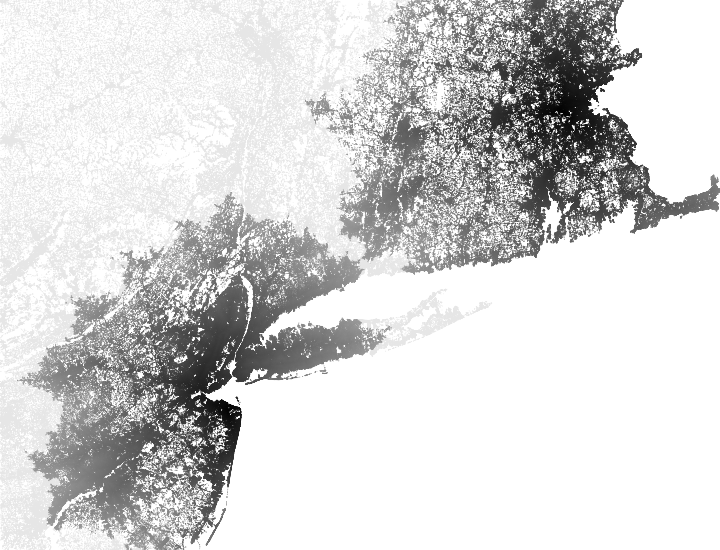
\includegraphics[width=2.0cm]{figs/incbi-road-ne/singleshot/example-bidijkstra.png}};

   % END LAZYSP

   % END LEMUR

   % top left side
   \node[fill=blue!10,draw=blue!20,rounded corners,align=center,minimum height=1.5cm,minimum width=1.8cm,inner sep=0pt] at (6.0,7.0) {};
   \node[fill=white,inner sep=0pt] at (6.0,7.0) {\includegraphics[width=1.4cm]{build/c-space-simple}};
   \node[font=\scriptsize] at (5.65,6.7) {$\mathcal{C}_{\mbox{\tiny free}}$};
   \draw[->] (6.0,6.25) -- (6.0,5.25) node [pos=0.55,fill=blue!5,align=center,inner sep=0pt] {\strut $\mathcal{C}$};

   %\node[inner sep=4pt] (cspace) at (3.3,7.0) {$\mathcal{C}$-Space};
   %\draw[->] (cspace) -- (3.3,5.25);

   % left side
   \draw[->] (0.5,2.0) -- (2.5,2.0);
   \node[fill=white,align=center,inner sep=2pt] at (0.5,2.0)
      {$q_{\ms{start}}$\\$q_{\ms{dest}}$};

   % right side
   \draw[->] (9.5,2.0) -- (11.3,2.0);
   \node[fill=white,align=center,inner sep=2pt] at (11.5,2.0)
      {$\xi$};

   \end{tikzpicture}
\end{frame}


%\begin{frame}
   %\frametitle{Talk Outline}
   %\begin{tikzpicture}[font=\small]
      %\tikzset{>=latex} % arrow heads
      %\draw[step=1,black!15,very thin,opacity=\gridopacity] (0,0) grid (12,8);

      %\node[fill=blue!15,minimum width=11cm] at (6,7.5) {\strut What to Optimize?};

      %\node[fill=black!3,minimum width=5cm,minimum height=3cm] (utility) at (3.25,5.6) {};
      %\node[anchor=north] at (utility.north) {\strut Maximizing Utility};
      %\node at (3.25,5.35) {\includegraphics[width=2.5cm]{build/pvx-utility-anytime}};

      %\node[fill=black!3,minimum width=5cm,minimum height=3cm] (family) at (8.75,5.6) {};
      %\node[anchor=north] at (family.north) {\strut Utility in C-Space Familes};
      %\node at (8.75,5.4) {\includegraphics[width=3.0cm]{build/multiple-sets}};

      %\node[fill=blue!15,minimum width=11cm] at (6,3.5) {\strut How to Optimize?};

      %\node[fill=black!3,minimum width=5cm,minimum height=3cm] (lazysp) at (3.25,1.6) {};
      %\node[anchor=north] at (lazysp.north) {\strut Lazy Pathfinding};
      %\node[draw=black!30,fill=white,inner sep=5pt] at (3.25,1.4) {
         %\includegraphics[width=3.8cm]{build/lazysp-icon}};

      %\node[fill=black!3,minimum width=5cm,minimum height=3cm] (ibid) at (8.75,1.6) {};
      %\node[anchor=north] at (ibid.north) {\strut Dynamic Pathfinding};
      %\node[draw=black!30,inner sep=0pt] at (8.75,1.4) {
         %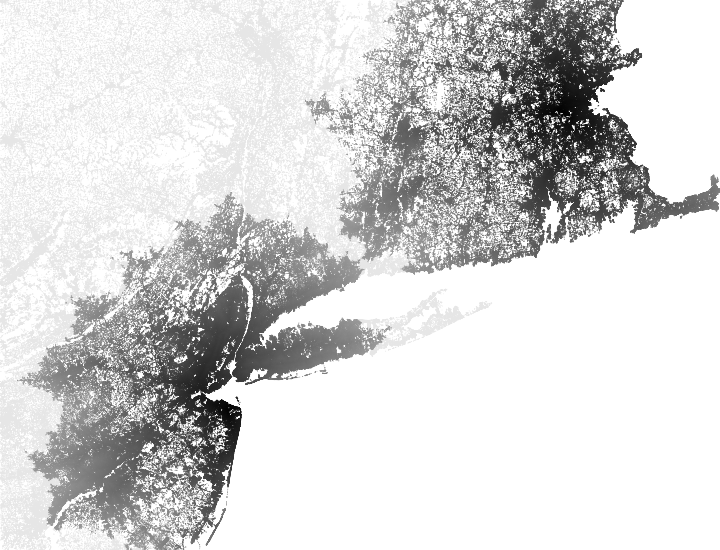
\includegraphics[width=2.9cm]{figs/incbi-road-ne/singleshot/example-bidijkstra.png}};

      %\only<2>
      %{
         %\draw[ultra thick] (utility.north west) rectangle (utility.south east);
      %}
      
   %\end{tikzpicture}
%\end{frame}

%\begin{frame}
%   \frametitle{Maximizing Utility in Motion Planning}
%   \begin{tikzpicture}[font=\small]
%      \tikzset{>=latex} % arrow heads
%
%      \draw[step=1,black!15,very thin,opacity=\gridopacity] (0,0) grid (12,8);
%
%      \node at ( 6,4) {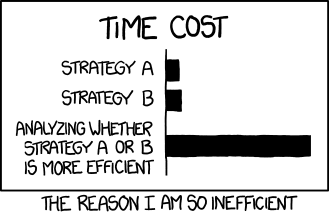
\includegraphics[width=5cm]{figs/xkcd-1445-efficiency.png}};
%      
%   \end{tikzpicture}
%\end{frame}

\begin{frame}
   \frametitle{Maximizing Utility in Motion Planning}
   \begin{tikzpicture}[font=\small]
      \tikzset{>=latex} % arrow heads

      \draw[step=1,black!15,very thin,opacity=\gridopacity] (0,0) grid (12,8);

      \only<1>{\node at (2.75,5.5) {\includegraphics{build/pvx-graph-build,drawempty}};}
      \only<2>{\node at (2.75,5.5) {\includegraphics{build/pvx-graph-build,drawaxes}};}
      \only<3>{\node at (2.75,5.5) {\includegraphics{build/pvx-graph-build,drawa}};}
      \only<4>{\node at (2.75,5.5) {\includegraphics{build/pvx-graph-build,drawab}};}
      \only<5>{\node at (2.75,5.5) {\includegraphics{build/pvx-graph-build,drawabxstar}};}
      \only<6>{\node at (2.75,5.5) {\includegraphics{build/pvx-graph-build,drawabxstarc}};}
      \only<7-8>{\node at (2.75,5.5) {\includegraphics{build/pvx-graph-build,drawabxstarcd}};}
      \only<9->{\node at (2.75,5.5) {\includegraphics{build/pvx-graph-build,drawabxstarcdutility}};}

      \only<3->{
      \node[fill=blue!5,draw=blue!10,rounded corners,align=center,anchor=north,minimum width=5cm] at (8.5,7.0) {
         \only<3>{$A_1$: a planner invocation}
         \only<4->{$A_1, A_2$: planner invocations}
         \only<6->{\\ $A_3$: an anytime planner}
         \only<7->{\\ $A_4$: a parameterized planner}};
      }

      \only<2->{
      \node[fill=blue!5,draw=blue!10,rounded corners,align=center] at (8.5,4.5) {
         $p$: planning cost incurred during invocation\\
         $x$: execution cost of resulting solution path};
      }
      \only<8->{
      \node[fill=blue!5,draw=blue!10,rounded corners,align=center,anchor=north] at (6,3.0) {
         $\arraycolsep=1.5pt \begin{array}{rc}
            U(p,x): & \mbox{real-valued utility function} \\
            & \mbox{which scores the invocation}
            \only<9->{\\ & \mbox{(isocontours shown)}}
         \end{array}$};
      }

      \only<8->{
      \node[anchor=west,font=\scriptsize] at (1.0,0.5) {\begin{minipage}{10cm}
      \hangindent=0.3cm \raggedright
         \PaperPortrait\; Burns, Ruml, and Do,
         ``Heuristic Search when Time Matters,''
         IJCAI 2013.
      \end{minipage}};
      }

   \end{tikzpicture}
\end{frame}

\begin{frame}
   \frametitle{Examples of Utility Functions}
   \begin{tikzpicture}[font=\small]
      \tikzset{>=latex} % arrow heads
      \draw[step=1,black!15,very thin,opacity=\gridopacity] (0,0) grid (12,8);


      \only<1->{
      \node at (1.92,6.5) {\includegraphics{build/pvx-sm-firstfeas}};
      \node[anchor=west] at (3.5,6.6) {\begin{minipage}{8cm}
         {\bf First Feasible} --

         Find a feasible solution as quickly as possible \\
         irrespective of its cost.
      \end{minipage}};
      }


      \only<2->{
      \node at (1.92,4.0) {\includegraphics{build/pvx-sm-pbudget}};
      \node[anchor=west] at (3.5,4.1) {\begin{minipage}{8cm}
         {\bf Planning Budget} --

         Return the lowest-cost path possible within a \\
         specified planning resource budget.
      \end{minipage}};
      }


      \only<3->{
      \node at (1.82,1.5) {\includegraphics{build/pvx-sm-xbudget}};
      \node[anchor=west] (boundedcost) at (3.5,1.6) {\begin{minipage}{8cm}
         {\bf Bounded Cost} --

         Find a solution as fast as possible within a \\
         specified path cost bound.
         
      \end{minipage}};
      \node[anchor=north,font=\scriptsize,below=-0.1cm of boundedcost.south] {\begin{minipage}{8cm}
      \hangindent=0.3cm \raggedright
         \PaperPortrait\; Stern et al,
         ``Potential-based Bounded-cost Search and Anytime Non-Parametric A*,''
         AI 2014.
      \end{minipage}};
      }
      

   \end{tikzpicture}
\end{frame}


\begin{frame}
   \frametitle{Algorithm Outline: Maximizing Utility over Paths}
   \begin{tikzpicture}[font=\small]
      \tikzset{>=latex} % arrow heads
      \draw[step=1,black!15,very thin,opacity=\gridopacity] (0,0) grid (12,8);

      \only<2>{
         \node[fill=blue!10,draw=blue!20,rounded corners,align=center] at (6,5)
         {
            Central assumption: planning cost is dominated by\\
            \emph{validating paths} (i.e. evaluating their cost).
         };
      }

      \only<3->{
      \node[fill=blue!5,rounded corners,anchor=north,minimum width=9.5cm,minimum height=3.6cm] (alg) at (6,7.75) {};
      \begin{scope} % highlights
         \clip[rounded corners] (alg.north west) rectangle (alg.south east);
         \only<3>{\node[fill=blue!15,anchor=north,minimum width=9.5cm,minimum height=0.5cm,below=0cm of alg.north] {};} % pinit
         \only<4>{\node[fill=blue!15,anchor=north,minimum width=9.5cm,minimum height=0.45cm,below=0.4cm of alg.north] {};} % iters
         \only<5,11,15>{\node[fill=blue!15,anchor=north,minimum width=9.5cm,minimum height=0.45cm,below=0.8cm of alg.north] {};} % pathset
         \only<6>{\node[fill=blue!15,anchor=north,minimum width=9.5cm,minimum height=0.9cm,below=1.2cm of alg.north] {};} % estimators
         \only<7,12,16>{\node[fill=blue!15,anchor=north,minimum width=9.5cm,minimum height=0.45cm,below=2.0cm of alg.north] {};} % argmin
         \only<8,17>{\node[fill=blue!15,anchor=north,minimum width=9.5cm,minimum height=0.45cm,below=2.35cm of alg.north] {};} % return
         \only<9,13>{\node[fill=blue!15,anchor=north,minimum width=9.5cm,minimum height=0.45cm,below=2.75cm of alg.north] {};} % eval
         \only<10,14>{\node[fill=blue!15,anchor=north,minimum width=9.5cm,minimum height=0.45cm,below=3.15cm of alg.north] {};} % updatep
      \end{scope}
      \node[left=0.1cm of alg.north,anchor=north] {\begin{minipage}{9cm}
         \begin{algorithmic}[1]
         \State $p_0 \leftarrow 0$
            \Comment planning cost incurred so far
         \only<4->{
         \For {iteration $i \in 1, 2, \dots$}
            \only<5->{
            \State $\Xi_i \leftarrow$ set of paths to consider at iteration $i$
            }%
            \only<6->{
            \State $\hat{x}_i : \Xi_i \rightarrow \mathbb{R}^+$
               \Comment execution cost estimator
            \State $\hat{p}_i : \Xi_i \rightarrow \mathbb{R}^+$
               \Comment additional planning cost estimator%
            }%
            \only<7->{
            \State $\xi_i = \argmax_{\xi \in \Xi_i}
               U\!\left( \; p_{i-1} \! + \! \hat{p}_i(\xi), \; \hat{x}_i(\xi) \; \right)$
               \label{line:outline-argmax}
            }%
            \only<8->{
            \State \Return $\xi_i$
               if $\xi_i$ fully evaluated, i.e. $\hat{p}(\xi) = 0$
            }%
            \only<9->{
            \State evaluate $\xi_i$
               \Comment incurs planning cost $\Delta p_i$
            }%
            \only<10->{
            \State $p_i \leftarrow p_{i-1} + \Delta p_i$
            }%
         \EndFor
         }
         \end{algorithmic}
      \end{minipage}};
      }

      \only<1-3>{\node at (3.5,2.0) {\includegraphics{build/cspace-utility-intro,start}};}
      \only<5-6>{\node at (3.5,2.0) {\includegraphics{build/cspace-utility-intro,candidatesa}};}
      \only<7-8>{\node at (3.5,2.0) {\includegraphics{build/cspace-utility-intro,candidatea}};}
      \only<9-10>{\node at (3.5,2.0) {\includegraphics{build/cspace-utility-intro,candidateaevaled}};}
      \only<11>{\node at (3.5,2.0) {\includegraphics{build/cspace-utility-intro,candidatesb}};}
      \only<12>{\node at (3.5,2.0) {\includegraphics{build/cspace-utility-intro,candidateb}};}
      \only<13-14>{\node at (3.5,2.0) {\includegraphics{build/cspace-utility-intro,candidatebevaled}};}
      \only<15>{\node at (3.5,2.0) {\includegraphics{build/cspace-utility-intro,candidatesfinal}};}
      \only<16->{\node at (3.5,2.0) {\includegraphics{build/cspace-utility-intro,candidatefinal}};}

      \only<3>{\node at (9.0,2.0) {\includegraphics{build/p-estimates-build,start}};}
      \only<4-6>{\node at (9.0,2.0) {\includegraphics{build/p-estimates-build,iterlabel}};}
      \only<7-8>{\node at (9.0,2.0) {\includegraphics{build/p-estimates-build,candidatea}};}
      \only<9>{\node at (9.0,2.0) {\includegraphics{build/p-estimates-build,candidateadelta}};}
      \only<10-11>{\node at (9.0,2.0) {\includegraphics{build/p-estimates-build,candidateaeval}};}
      \only<12>{\node at (9.0,2.0) {\includegraphics{build/p-estimates-build,candidateb}};}
      \only<13>{\node at (9.0,2.0) {\includegraphics{build/p-estimates-build,candidatebdelta}};}
      \only<14>{\node at (9.0,2.0) {\includegraphics{build/p-estimates-build,candidatebeval}};}
      \only<15-16>{\node at (9.0,2.0) {\includegraphics{build/p-estimates-build,prefinal}};}
      \only<17>{\node at (9.0,2.0) {\includegraphics{build/p-estimates-build,final}};}

   \end{tikzpicture}
\end{frame}

\begin{frame}
   \frametitle{Aside: Simplified Bidirectional RRT-Connect}
   \begin{tikzpicture}[font=\small]
      \tikzset{>=latex} % arrow heads
      \draw[step=1,black!15,very thin,opacity=\gridopacity] (0,0) grid (12,8);

      \node[fill=blue!5,rounded corners,anchor=north,minimum width=9.5cm,minimum height=3.6cm] (alg) at (6,7.75) {};
      \begin{scope} % highlights
         \clip[rounded corners] (alg.north west) rectangle (alg.south east);
         %\only<2>{\node[fill=blue!15,anchor=north,minimum width=9.5cm,minimum height=0.5cm,below=0cm of alg.north] {};} % pinit
         %\only<3>{\node[fill=blue!15,anchor=north,minimum width=9.5cm,minimum height=0.45cm,below=0.4cm of alg.north] {};} % iters
         \only<4>{\node[fill=blue!15,anchor=north,minimum width=9.5cm,minimum height=0.45cm,below=0.8cm of alg.north] {};} % pathset
         %\only<5>{\node[fill=blue!15,anchor=north,minimum width=9.5cm,minimum height=0.9cm,below=1.2cm of alg.north] {};} % estimators
         \only<5->{\node[fill=blue!15,anchor=north,minimum width=9.5cm,minimum height=0.45cm,below=2.0cm of alg.north] {};} % argmin
         %\only<7,16>{\node[fill=blue!15,anchor=north,minimum width=9.5cm,minimum height=0.45cm,below=2.35cm of alg.north] {};} % return
         %\only<8,12>{\node[fill=blue!15,anchor=north,minimum width=9.5cm,minimum height=0.45cm,below=2.75cm of alg.north] {};} % eval
         %\only<9,13>{\node[fill=blue!15,anchor=north,minimum width=9.5cm,minimum height=0.45cm,below=3.15cm of alg.north] {};} % updatep
      \end{scope}
      \node[left=0.1cm of alg.north,anchor=north] {\begin{minipage}{9cm}
         \begin{algorithmic}[1]
         \State $p_0 \leftarrow 0$
            \Comment planning cost incurred so far
         \For {iteration $i \in 1, 2, \dots$}
            \State $\Xi_i \leftarrow$ set of paths to consider at iteration $i$
            \State $\hat{x}_i : \Xi_i \rightarrow \mathbb{R}^+$
               \Comment execution cost estimator
            \State $\hat{p}_i : \Xi_i \rightarrow \mathbb{R}^+$
               \Comment additional planning cost estimator
            \State $\xi_i = \argmax_{\xi \in \Xi_i}
               U\!\left( \; p_{i-1} \! + \! \hat{p}_i(\xi), \; \hat{x}_i(\xi) \; \right)$
               \label{line:outline-argmax}
            \State \Return $\xi_i$
               if $\xi_i$ fully evaluated, i.e. $\hat{p}(\xi) = 0$
            \State evaluate $\xi_i$
               \Comment incurs planning cost $\Delta p_i$
            \State $p_i \leftarrow p_{i-1} + \Delta p_i$
         \EndFor
         \end{algorithmic}
      \end{minipage}};

      \only<1>{\node at (3.7,2.0) {\includegraphics{build/rrt-build,stonly}};}
      \only<2>{\node at (3.7,2.0) {\includegraphics{build/rrt-build,stexisting}};}
      \only<3>{\node at (3.7,2.0) {\includegraphics{build/rrt-build,target}};}
      \only<4-5>{\node at (3.7,2.0) {\includegraphics{build/rrt-build,otherpaths}};}
      \only<6->{\node at (3.7,2.0) {\includegraphics{build/rrt-build,all}};}
      
      \only<6->{\node at (8.7,2.0) {\includegraphics{build/pvx-rrt}};}

      \only<7>{
         \node[fill=white,opacity=0.8,text opacity=1.0,inner sep=5pt,rounded corners] at (6,4.2) {
         \begin{tikzpicture}
         \node[fill=black!5,draw=black!15,rounded corners,align=center]
            {RRT-Connect implicitly maximizes utility at each iteration\\
            using the first-feasible utility function.};
         \end{tikzpicture}
         };
      }

   \end{tikzpicture}
\end{frame}

\begin{frame}
   \frametitle{Maximizing Utility over Roadmaps}
   \begin{tikzpicture}[font=\small]
      \draw[step=1,black!15,very thin,opacity=\gridopacity] (0,0) grid (12,8);

      %\node[fill=blue!15,minimum width=11cm] at (6,7.5) {\strut How to Optimize?};
      %\node[fill=blue!15,minimum width=11cm] at (6,6.75) {\strut What to Optimize?};

      \node[fill=blue!5,rounded corners,anchor=north,minimum width=9.5cm,minimum height=3.6cm] (alg) at (6,7.75) {};
      \begin{scope} % highlights
         \clip[rounded corners] (alg.north west) rectangle (alg.south east);
         %\only<2>{\node[fill=blue!15,anchor=north,minimum width=9.5cm,minimum height=0.5cm,below=0cm of alg.north] {};} % pinit
         %\only<3>{\node[fill=blue!15,anchor=north,minimum width=9.5cm,minimum height=0.45cm,below=0.4cm of alg.north] {};} % iters
         \only<2-3>{\node[fill=blue!15,anchor=north,minimum width=9.5cm,minimum height=0.45cm,below=0.8cm of alg.north] {};} % pathset
         %\only<5>{\node[fill=blue!15,anchor=north,minimum width=9.5cm,minimum height=0.9cm,below=1.2cm of alg.north] {};} % estimators
         %\only<5->{\node[fill=blue!15,anchor=north,minimum width=9.5cm,minimum height=0.45cm,below=2.0cm of alg.north] {};} % argmin
         %\only<7,16>{\node[fill=blue!15,anchor=north,minimum width=9.5cm,minimum height=0.45cm,below=2.35cm of alg.north] {};} % return
         %\only<8,12>{\node[fill=blue!15,anchor=north,minimum width=9.5cm,minimum height=0.45cm,below=2.75cm of alg.north] {};} % eval
         %\only<9,13>{\node[fill=blue!15,anchor=north,minimum width=9.5cm,minimum height=0.45cm,below=3.15cm of alg.north] {};} % updatep
      \end{scope}
      \node[left=0.1cm of alg.north,anchor=north] {\begin{minipage}{9cm}
         \begin{algorithmic}[1]
         \State $p_0 \leftarrow 0$
            \Comment planning cost incurred so far
         \For {iteration $i \in 1, 2, \dots$}
            \State $\Xi_i \leftarrow$ set of paths to consider at iteration $i$
            \State $\hat{x}_i : \Xi_i \rightarrow \mathbb{R}^+$
               \Comment execution cost estimator
            \State $\hat{p}_i : \Xi_i \rightarrow \mathbb{R}^+$
               \Comment additional planning cost estimator
            \State $\xi_i = \argmax_{\xi \in \Xi_i}
               U\!\left( \; p_{i-1} \! + \! \hat{p}_i(\xi), \; \hat{x}_i(\xi) \; \right)$
               \label{line:outline-argmax}
            \State \Return $\xi_i$
               if $\xi_i$ fully evaluated, i.e. $\hat{p}(\xi) = 0$
            \State evaluate $\xi_i$
               \Comment incurs planning cost $\Delta p_i$
            \State $p_i \leftarrow p_{i-1} + \Delta p_i$
         \EndFor
         \end{algorithmic}
      \end{minipage}};

      \only<3->{
         \fill[white,path fading=fade down] (1,6.5) rectangle (11,6.0);
         \fill[white] (1,6.0) rectangle (11,4);

         \node at (2.25,3.25) {\includegraphics[width=3.0cm]{build/roadmap-stack-onramps}};

         \node[anchor=north,fill=black!3,rounded corners] at (8,5.5) {\begin{minipage}{7cm}
            \raggedright
         
            Focus: Roadmap methods

            \medskip
            Advantages:
            \begin{itemize}
            \item Well-studied asymptotic completeness\\
               and optimality properties
            \item Easy to progressively densify
            \item Common structure across queries\\
               (can load roadmaps from disk)
            \end{itemize}
         \end{minipage}};
      }
      
   \end{tikzpicture}
\end{frame}

\begin{frame}
   \frametitle{Maximizing Linear Utilities with Additive Estimators}
   \begin{tikzpicture}[font=\small]
      \draw[step=1,black!15,very thin,opacity=\gridopacity] (0,0) grid (12,8);
      \tikzset{>=latex} % arrow heads

      %\node[fill=blue!15,minimum width=11cm] at (6,7.5) {\strut How to Optimize?};
      %\node[fill=blue!15,minimum width=11cm] at (6,6.75) {\strut What to Optimize?};

      \node[fill=blue!5,rounded corners,anchor=north,minimum width=9.5cm,minimum height=3.6cm] (alg) at (6,7.75) {};
      \begin{scope} % highlights
         \clip[rounded corners] (alg.north west) rectangle (alg.south east);
         %\only<2>{\node[fill=blue!15,anchor=north,minimum width=9.5cm,minimum height=0.5cm,below=0cm of alg.north] {};} % pinit
         %\only<3>{\node[fill=blue!15,anchor=north,minimum width=9.5cm,minimum height=0.45cm,below=0.4cm of alg.north] {};} % iters
         \only<3>{\node[fill=blue!15,anchor=north,minimum width=9.5cm,minimum height=0.45cm,below=0.8cm of alg.north] {};} % pathset
         \only<3>{\node[fill=blue!15,anchor=north,minimum width=9.5cm,minimum height=0.9cm,below=1.10cm of alg.north] {};} % estimators
         \only<4,8->{\node[fill=blue!15,anchor=north,minimum width=9.5cm,minimum height=0.45cm,below=2.0cm of alg.north] {};} % argmin
         %\only<7,16>{\node[fill=blue!15,anchor=north,minimum width=9.5cm,minimum height=0.45cm,below=2.35cm of alg.north] {};} % return
         \only<5-7>{\node[fill=blue!15,anchor=north,minimum width=9.5cm,minimum height=0.45cm,below=2.75cm of alg.north] {};} % eval
         %\only<9,13>{\node[fill=blue!15,anchor=north,minimum width=9.5cm,minimum height=0.45cm,below=3.15cm of alg.north] {};} % updatep
      \end{scope}
      \node[left=0.1cm of alg.north,anchor=north] {\begin{minipage}{9cm}
         \begin{algorithmic}[1]
         \State $p_0 \leftarrow 0$
            \Comment planning cost incurred so far
         \For {iteration $i \in 1, 2, \dots$}
            \State $\Xi_i \leftarrow$ set of paths to consider at iteration $i$
            \State $\hat{x}_i : \Xi_i \rightarrow \mathbb{R}^+$
               \Comment execution cost estimator
            \State $\hat{p}_i : \Xi_i \rightarrow \mathbb{R}^+$
               \Comment additional planning cost estimator
            \only<1-8>{\State $\xi_i = \argmax_{\xi \in \Xi_i}
               U\!\left( \; p_{i-1} \! + \! \hat{p}_i(\xi), \; \hat{x}_i(\xi) \; \right)$
               \label{line:outline-argmax}}%
            \only<9->{\State $\xi_i = \argmax_{\xi \in \Xi_i}
               U\!\left( \; \hat{p}_i(\xi), \; \hat{x}_i(\xi) \; \right)$
               \label{line:outline-argmax}}%
            \State \Return $\xi_i$
               if $\xi_i$ fully evaluated, i.e. $\hat{p}(\xi) = 0$
            \State evaluate $\xi_i$
               \Comment incurs planning cost $\Delta p_i$
            \State $p_i \leftarrow p_{i-1} + \Delta p_i$
         \EndFor
         \end{algorithmic}
      \end{minipage}};

      \only<2->{
         \node[fill=black!5,draw=black!20,rounded corners] at (3.0,3.0)
         {\begin{minipage}{4.9cm}
            We consider \emph{linear utility functions}:
            \vspace{-0.2cm}
            \[
               -U(p,x) = \lambda \, p + (1 - \lambda) \, x
            \]
         \end{minipage}};
      }
      \only<10->{
         \node[fill=black!5,draw=black!20,rounded corners] at (8.7,3.0) {\begin{minipage}{5.6cm}
            We consider \emph{additive estimators}:
            \vspace{-0.2cm}
            \[
               \xi: \mbox{path on a roadmap graph } G
            \]
            \vspace{-0.5cm}
            \[
               \grave{p}_i(\xi) = \sum_{e \in \xi} \hat{p}_i(e)
               \;\;\mbox{and}\;\;
               \hat{x}_i(\xi) = \sum_{e \in \xi} \hat{x}_i(e)
            \]
         \end{minipage}};
      }

      \only<3>{\node at (8.5,2) {\includegraphics[width=3.75cm]{build/pvx-linear-discounting-build,beforeeval}};}
      \only<4>{\node at (8.5,2) {\includegraphics[width=3.75cm]{build/pvx-linear-discounting-build,selectcandidate}};}
      \only<5>{\node at (8.5,2) {\includegraphics[width=3.75cm]{build/pvx-linear-discounting-build,newcandidate}};}
      \only<6>{\node at (8.5,2) {\includegraphics[width=3.75cm]{build/pvx-linear-discounting-build,newshared}};}
      \only<7-8>{\node at (8.5,2) {\includegraphics[width=3.75cm]{build/pvx-linear-discounting-build,newother}};}
      \only<9>{\node at (8.5,2) {\includegraphics[width=3.75cm]{build/pvx-linear-discounting-build,newaxes}};}

      \only<11->{
         \draw[->,very thick] (5.65,1.9) -- (5.65,1.4);
      
         \node[fill=black!5,draw=black!20,rounded corners] at (5.8,0.8) {\begin{minipage}{5cm}
            Shortest path problem with:
            \vspace{-0.2cm}
            \[
               w_i(e) = \lambda_U \, \hat{p}_i(e) + (1 - \lambda_U) \, \hat{x}_i(e)
            \]
         \end{minipage}};
      }
      
   \end{tikzpicture}
\end{frame}


% all this data cumulative over the multistep-prescribed problem

\pgfplotstableread{
lambda searchmean evalmean
lam00 0.13717146918 1.566855428440001
lam20 0.13591121493999997 1.5040972085999997
lam50 0.12633906594 1.3774433666
lam80 0.11458146473999997 1.2423356615
lam99 0.10054155609999996 0.9362152972200001
}{\datasvetimeherbbinnom}

\pgfplotstableread{
lambda searchmean evalmean
lam00 0.9183584741400002 4.73433351068
lam20 0.8734410922000001 4.4884742077799995
lam50 0.82153580024 4.091855509880002
lam80 0.75752757384 3.39455290978
lam99 0.7430251334600001 3.0377397256199994
}{\datasvetimeworkcell}

\begin{frame}
   \frametitle{Search vs. Evaluation Planning Time Comparison}
   \begin{tikzpicture}[font=\small]
      \draw[step=1,black!15,very thin,opacity=\gridopacity] (0,0) grid (12,8);
      \tikzset{>=latex} % arrow heads

      \node at (8.2,7.4) {
         \protect\tikz{\protect\node[fill=red!20,draw=black]{};}\;graph search vs.
         \protect\tikz{\protect\node[fill=blue!20,draw=black]{};}\;edge evaluation
      };

      \node[fill=black!5,draw=black!20,rounded corners,minimum width=11cm,minimum height=3cm] at (6.0,5.5) {};

      \node at ( 2.5,5.5) {
         \includegraphics[width=1.7cm]{figs/herbbin/step0cropped.png}
         \includegraphics[width=1.7cm]{figs/herbbin/step01cropped.png}};

      \begin{scope}[shift={(5.5,5.0)}]
      \begin{axis}[
         width=7.0cm,
         height=3.2cm,
         xbar stacked,
         bar width=7,
         %xmin=0,xmax=10,
         xmin=0,
         %xtick pos=bottom,
         %symbolic y coords={E, F, R, A, B, W, P},
         %yticklabels from table={\datasvetimeherbbinnom}{lambda},
         yticklabels={$0.00$,,,,$0.99$},
         ylabel={$\lambda$},
         ytick=data,
         %ytick pos=left,
         xmajorgrids,
         xmajorticks=true,
         %ticklabel style={font=\footnotesize},
         enlarge y limits={abs=0.2cm},
         ylabel near ticks,
         ylabel shift=-0.5cm,
         ylabel style={rotate=-90},
         xlabel={Average S/E Planning Time (s)},
         xlabel near ticks,
         ] 
      %\node[circle,fill=white,inner sep=1pt,text=black!40] at (axis cs:40,-5.6) {\scriptsize 40};
      %\node[circle,fill=white,inner sep=1pt,text=black!40] at (axis cs:60,-5.6) {\scriptsize 60};
      %\node[circle,fill=white,inner sep=1pt,text=black!40] at (axis cs:80,-5.6) {\scriptsize 80};
      \addplot[color=black,fill=red!20]
         table[y expr=-\coordindex,x=searchmean]
         {\datasvetimeherbbinnom};
      \addplot[color=black,fill=blue!20]
         table[y expr=-\coordindex,x=evalmean]
         {\datasvetimeherbbinnom};
      \end{axis}
      \end{scope}

      \node[fill=black!5,draw=black!20,rounded corners,minimum width=11cm,minimum height=3cm] at (6.0,2.2) {};

      \node at ( 2.5,2.2) {
         \includegraphics[width=3.5cm]{videos/workcell-cropped.png}};

      \begin{scope}[shift={(5.5,1.7)}]
      \begin{axis}[
         width=7.0cm,
         height=3.2cm,
         xbar stacked,
         bar width=7,
         %xmin=0,xmax=10,
         xmin=0,
         %xtick pos=bottom,
         %symbolic y coords={E, F, R, A, B, W, P},
         %yticklabels from table={\datasvetimeherbbinnom}{lambda},
         yticklabels={$0.00$,,,,$0.99$},
         ylabel={$\lambda$},
         ytick=data,
         %ytick pos=left,
         xmajorgrids,
         xmajorticks=true,
         %ticklabel style={font=\footnotesize},
         enlarge y limits={abs=0.2cm},
         ylabel near ticks,
         ylabel shift=-0.5cm,
         ylabel style={rotate=-90},
         xlabel={Average S/E Planning Time (s)},
         xlabel near ticks,
         ] 
      %\node[circle,fill=white,inner sep=1pt,text=black!40] at (axis cs:40,-5.6) {\scriptsize 40};
      %\node[circle,fill=white,inner sep=1pt,text=black!40] at (axis cs:60,-5.6) {\scriptsize 60};
      %\node[circle,fill=white,inner sep=1pt,text=black!40] at (axis cs:80,-5.6) {\scriptsize 80};
      \addplot[color=black,fill=red!20]
         table[y expr=-\coordindex,x=searchmean]
         {\datasvetimeworkcell};
      \addplot[color=black,fill=blue!20]
         table[y expr=-\coordindex,x=evalmean]
         {\datasvetimeworkcell};
      \end{axis}
      \end{scope}

   \end{tikzpicture}
\end{frame}
